\chapter{Design und Konzeption}
Nach der Analyse der Aufgabenstellung und der Erarbeitung des Knowhows im Bereich von Scala und des Lift Frameworks ging es an Design und Konzeption. In dieser Phase entstanden auf der Basis von \ref{konzept:usecase} \titleref{konzept:usecase} die in der Aufgabenstellung definierten Konzepte der Benutzerrollen, Navigationskonzept und der Prozesse. Als Basis f\"ur die Implementation dient zum Ende \ref{design:erm} \titleref{design:erm} und \ref{design:architektur} \titleref{design:architektur}
\section{Use Cases Beschreibung}\label{konzept:usecase}
 \begin{figure}[H]
  	\centering
    	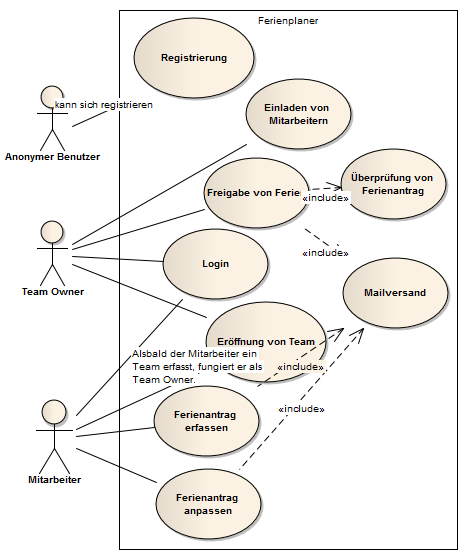
\includegraphics[width=13cm]{images/usecases}
 	\caption{Use Case Diagramm}
\end{figure}
\subsection{Aktoren}
\subsubsection{Mitarbeiter} sind registrierte Benutzer und k\"onnen von Team Ownern zu den entsprechenden Teams hinzugef\"ugt werden. 
\subsubsection{Owner - Team Owner} sind grunds\"atzlich auch Mitarbeiter, die allerdings ein eigenes Team administrieren und f\"ur dieses (es k\"onnen auch mehrere sein) deshalb zus\"atzliche Kompetenzen besitzen.

\subsection{Beschreibung der Use Cases}
\subsubsection{Projekt er\"offnen}
Nach dem Login erfasst der Administrator (Project Manager, Teamleiter, usw.) f\"ur sein Team ein Projekt. Grunds\"atzlich geh\"ort ein Projekt mehreren Administratoren, in einem 2. Projekt wird die zus\"atzliche M\"oglichkeit implementiert, anderen Benutzer Administrator-Rechte f\"urs eigene Projekt zu geben.

\subsubsection{Mitarbeiter in Projekt erfassen}
Projekte alleine sind leere ''Beh\"alter'' f\"ur Mitarbeiter. Um Mitarbeiter ins eigene Projekt zu nehmen, sucht der Administrator nach einem bestehenden User. Sofern es den gesuchten Benutzer im System noch nicht gibt, wird er durch den Administrator neu erfasst. Der neu erfasste Benutzer wird mittels Mail auf diese Aktion aufmerksam gemacht.

\subsubsection{Ferienw\"unsche bearbeiten}
Die vom Mitarbeiter erfassten Ferien k\"onnen durch den Administrator bez\"uglich Status und Termin ver\"andert werden. Die Bewilligung von Ferien wird mittels des Status confirmed / best\"atigt erteilt. Ansonsten gibt es folgende M\"oglichkeiten:
\begin{itemize}
\item erw\"unscht - requested
\item abgelehnt - rejected
\item best\"atigt - confirmed
\end{itemize}

\subsubsection{Ferienwunsch erfassen}
Der Mitarbeiter kann seine Ferienw\"unsche pro Projekt erfassen. Diese befinden sich zu Beginn im Status ''requested'' und k\"onnen vom Administrator in die Status ''rejected'' und ''confirmed'' ge\"andert werden.

\subsubsection{Ferienwunsch bearbeiten}
Sollte ein Ferienwunsch abgelehnt werden, kann er erneut bearbeitet werden, was eine erneute Anfrage beim Administrator zur Folge hat.

\section{Rollen-Konzept}\label{konzept:rollen}
Im Grunde handelt es sich bei dem Ferienplaner um einen Prototypen ohne eigentlichen Business Case im Hintergrund. Aus diesem Grund sehe ich als Anfang nur 2 Rollen vor. Zum einen ist es der Anonyme Benutzer, der zwar die Webseite Besuchen kann, sich f\"ur die weiteren Schritte allerdings registrieren muss, zum anderen ist es der Registrierte Benutzer, der nicht nur Ferien erfassen, sondern auch eigene Teams mit eigenen Mitarbeitern bilden kann. Als Business Case k\"onnte ich mir vorstellen, dass es eine Trennung des Owners vom Mitarbeiter gibt, und daf\"ur spezielle Bedingungen (z.B. Bezahlung, etc.) erf\"ullt werden m\"ussen.
\subsection{Anonymous}
Folgende Funktionalit\"aten stehen dem Anonymous zur Verf\"ugung:
\begin{itemize}
\item Ansicht von \"offentlichen Seiten
\item Registrierung
\end{itemize}

\subsection{Registrierte Benutzer}
Nebst den Funktionen des Anonymous stehen dem Registrierten Benutzer folgende Dinge zur Auswahl:
\begin{itemize}
\item Login
\item Administration von Teams und Zuweisung von Mitarbeitern
\item Einladen von Mitarbeitern
\item Erfassen von Ferien f\"ur Teams welchen der Registrierte Benutzer angeh\"ort.
\end{itemize}

\subsection{Optional Aufteilung der Registrierten Benutzer}
Bei allf\"alligem Business Case best\"unde die M\"oglichkeit, die Rolle des Registrierten Benutzers in Mitarbeiter und Team Owner aufzuteilen. In diesem Falle h\"atte man die M\"oglichkeit, bestimmte Richtlinien (Zahlungsrichtlinien, etc.) zu errichten. Als Beispiel w\"urden die Rollen folgendermassen aussehen:
\subsubsection{Mitarbeiter}
Folgende Funktionalit\"aten stehen dem Mitarbeiter zur Verf\"ugung:
\begin{itemize}
\item Erfassen von Ferien f\"ur Teams welchen der Registrierte Benutzer angeh\"ort.
\end{itemize}

\subsubsection{Team Owner}
Zus\"atzlich zu den Funktionen des Mitarbeiters kann der Team Owner folgendes tun:
\begin{itemize}
\item Administration von Teams und Zuweisung von Mitarbeitern
\item Einladen von Mitarbeitern
\end{itemize}

\section{Prozesse}\label{konzept:prozesse}
\subsection{Person registrieren}
 \begin{figure}[H]
  	\centering
    	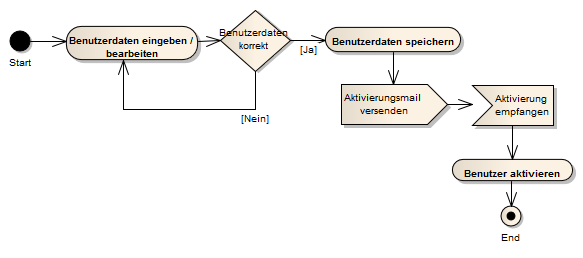
\includegraphics[width=15cm]{images/process_registration}
 	\caption{Prozess Member Administration Webpage}
\end{figure}

\subsection{Ferien beantragen, planen}\label{prozess:ferien}
 \begin{figure}[H]
  	\centering
    	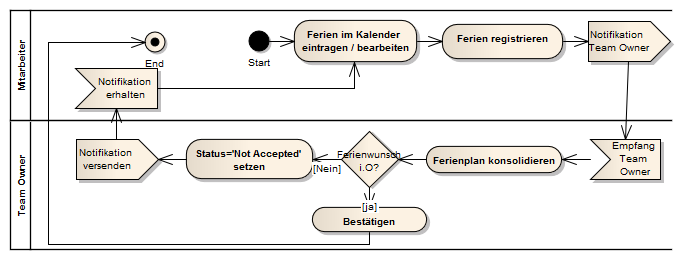
\includegraphics[width=15cm]{images/process_vacation}
 	\caption{Prozess Ferien beantragen, planen}
\end{figure}


\subsection{Team administrieren}\label{prozess:team}
 \begin{figure}[H]
  	\centering
    	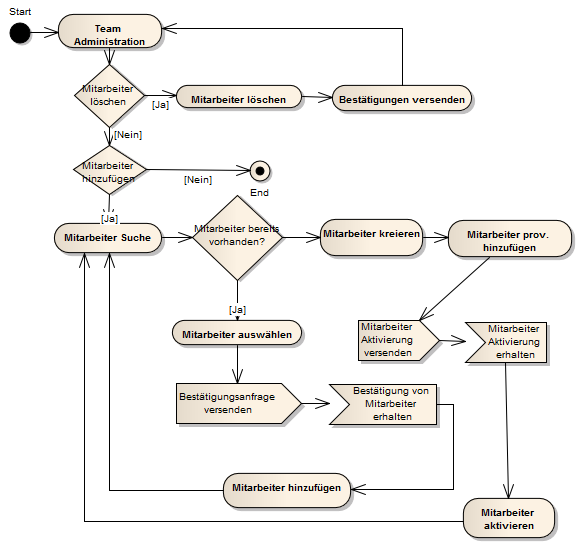
\includegraphics[width=15cm]{images/process_team_administration}
 	\caption{Prozess Member Administration Webpage}
\end{figure}

\section{Navigations-Konzept}\label{konzept:navigation}
 \begin{figure}[H]
  	\centering
    	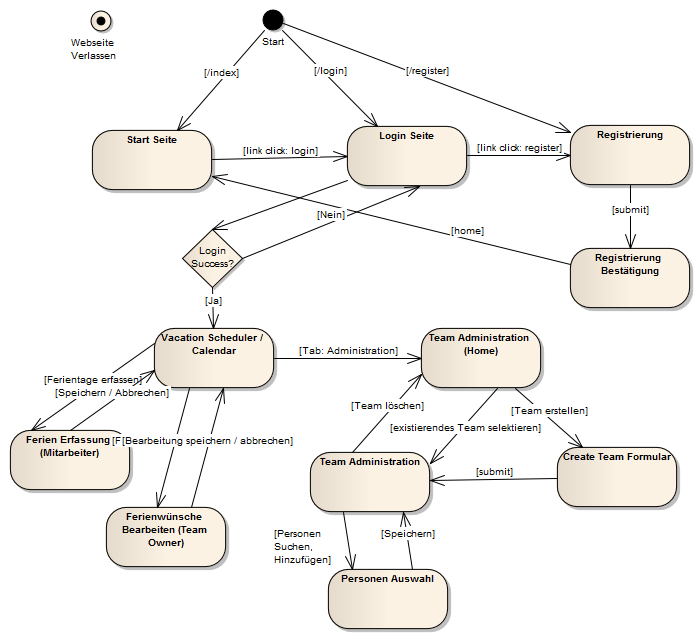
\includegraphics[width=13cm]{images/navigation_process}
 	\caption{Navigation Webpage}
\end{figure}

\section{Datenbank-Schema}\label{design:erm}

\subsection{Entity Relationship Model}
\begin{landscape}
 \begin{figure}
  	\centering
    	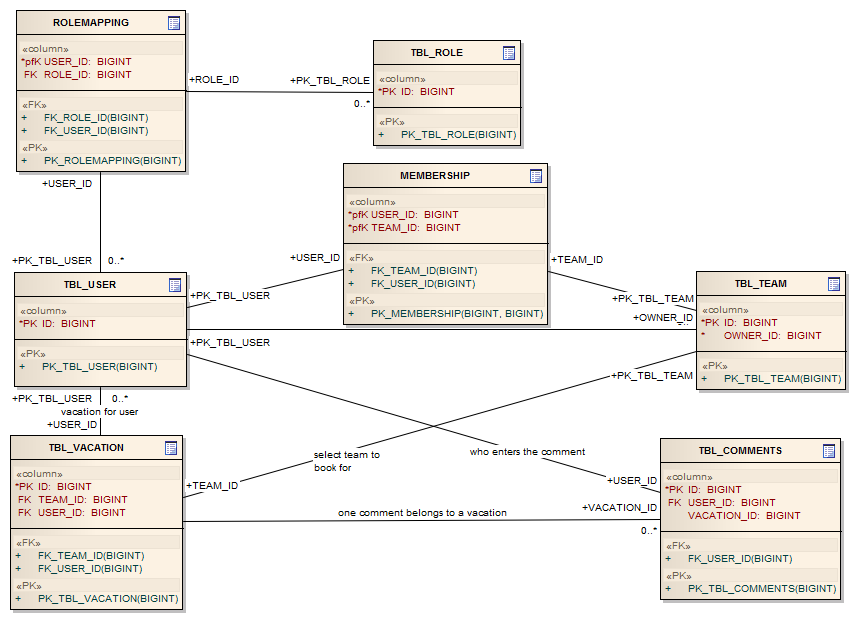
\includegraphics[width=19cm]{images/erm}
        	\caption{Entity Relationship Model}
\end{figure}
\end{landscape}
\subsection{Beschreibung}
Das Entity Relationship Model zeigt alle Tabellen, wie sieauf Ebene der Datenbank geplant sind. Many-to-Many Beziehungen sind also bereits aufgel\"ost. 

\subsubsection{User und Rollen}
Beginnen wir mit den Tabellen User und Rollen: F\"ur die Modellierung der Rollen gibt es meines Erachtens zwei vertretbare Alternativen. Erstens wie hier im ERM aufgezeigt, werden die Rollen via eine Join Table dem User zugewiesen. Die Erweiterung davon w\"are dann eine Zus\"atzlichen Self-Join auf der Tabelle TBL\_ROLE, damit man eine Hierarchie der Rollen abbilden kann, und Rollen den Benutzern auch in Gruppen zuweisen kann. Aufgrund der zus\"atzlichen Komplexit\"atsstufe habe ich mich f\"ur Variante eins entschieden.

\subsubsection{Teammitgliedschaft, Membership}
Die Zuteilung von Membern zu Teams muss ebenfalls \"uber eine Many-to-Many Assoziation realisiert werden. Im Diagramm ersichtlich an der Tabelle MEMBERSHIP. 

\subsubsection{Teamzugeh\"origkeit}
Im von mir modelierten einfacheren Fall, bei dem ein Team nur einem Verantwortlichen zugeteilt wird, wird die Beziehung zwischen TBL\_TEAM und TBL\_USER mittels einer One-To-Many Relation hergestellt. Nebst der Einfachheit hat dies den Nachteil, dass Ferien nur vom Ersteller und Team-Owner bewilligt werden k\"onnen, er kann also keine Stellvertreter daf\"ur nominieren. 

\subsubsection{Ferien}
Ferien werden als Eintr\"age in der Tabelle TBL\_VACATION definiert. Die Beziehung zu TBL\_USER ist relativ einleuchten, da diese immer einem Teilnehmer zugeordnet werden. Die Relation zu TBL\_TEAM kommt daher, weil ich Ferien immer \"fur ein spezifisches Team erfassen muss. Ob das dann manuell durch den Benutzer oder Applikatorisch f\"ur alle Teams durchgef\"uhrt wird, sei dahin gestellt. Jedenfalls, sofern ein Benutzer mehreren Teams zugeordnet ist, m\"ussen f\"ur all diese Teams Ferien-Records vorhanden sein.